\section{Theoretische und Technische Grundlagen}

In diesem Kapitel werden die technischen Grundlagen des Projektes, die zur Umsetzung nötig sind beschrieben.

\subsection{Robotik} % Manuel ca. 8
% Farbe die angibt welchen Status der folgende Abschnitt hat:
\color{finishing}
% Eigentlicher Text:
Die Robotik beschäftigt sich mit dem Entwurf, der Konstruktion sowie der Programmierung, Steuerung und dem Betrieb 
von Robotern \newline [http://wirtschaftslexikon.gabler.de/Definition/robotik.html]. Dabei umfasst die Robotik eine Vielzahl 
von Fachgebieten wie der Elektrotechnik, dem Maschienenbau, der Informatik sowie der Biologie und der Medizin.
\subsubsection{Roboter}
% Farbe die angibt welchen Status der folgende Abschnitt hat:
\color{finishing}
% Eigentlicher Text:
Was im Kontext der Robotik unter einem Roboter zu verstehen ist, ist gar nicht so einfach darzulegen, da es in Tat keine allgemein anerkannte Definition dieses Begriffs gibt, die seiner üblichen Verwendung entspricht [Mobile Roboter - 2].
\newline
Auch ohne eine vollkommen allgemeingültige und präzise Beschreibung eines Roboters zu sein, soll hier die VDI-Richtline 2860 einen Eindruck darüber vermitteln, was in der Robotik mit Roboter gemeint ist. \newline
Die VDI-Richtline 2860 von 1990 definiert einen Roboter wie folgt:
\vspace{2mm}
\newline
>>\textit{Ein Roboter ist ein frei und wieder programmierbarer, multifunktio-
naler Manipulator mit mindestens drei unabhängigen Achsen, um Ma-
terialien, Teile, Werkzeuge oder spezielle Geräte auf programmierten,
variablen Bahnen zu bewegen zur Erfüllung der verschiedensten Auf-
gaben.}<<
\vspace{2mm}
\newline
Auch wenn diese Definition einige grundlegenden Eigenschaften eines Roboters darlegt, beschreibt diese Definition den Begriff des Roboters im industriellen Kontext und trifft hauptsächlich auf stationäre Industrieroboter zu, wie sie in der Automobilfertigung beispielsweise als Schweiß- oder Lackierroboter verwendet werden. Die genannten programmierten Bahnen sind dort möglich, weil die Arbeitsprozess und die Umgebung auf den Roboter zugeschnitten und vollständig bekannt sind [MR 2]. \newline
Im Gegensatz dazu trifft dieser Aspekt auf mobile Roboter nicht zu, sich diese meist in einer unbekannten, unsttrukturierten und dynamischen Umgebung bewegen.
\subsubsection{Mobile Roboter}
% Farbe die angibt welchen Status der folgende Abschnitt hat:
\color{process}
% Eigentlicher Text:
Mobile Roboter bewegen sich selbständig duch eine sich meist ständig ändernde Umwelt, so dass alle ihre Aktionen von ihrer aktuellen Umgebung abhängen und diese erst zum Zeitpunkt der Ausführung dieser Aktionen bekannt ist im Detail. Dieser grundsätzliche Unterschied zu stationären Robotern macht es unerlässlich das mobile Roboter ihre Umgebung mittels Sensoren
erfassen, diese Sensordaten auswerten und auf Grundlage dessen ihre nächsten Aktionen planen.

der Hinsicht, 
Diese macht es notwendig das die Roboter ihre Umgebung erfassen und wahrnehmen können um auf Veränderungen wie bespielsweise Hindernisse reagieren zu können. \newline
...
\newline
Zu den Vertretern mobiler Roboter zählen zum Beispiel Service-Roboter, Erkundungsroboter und Humanoide Roboter.
Im Folgenden werden einige Beispielefür mobile Roboter dargelegt:
\begin{itemize}
	\item{\textbf{Shakey:}} Shakey war ein mobiler Roboter der von 1966 bis 1972 an der am Stanford Research Institute entwickelt wurde. Seine Entwicklung leistete wichtige Beiträge für die Robotik sowie in der KI-Forschung im Bereich der Handlungsplanung und dem selbständigen Lernen [MR 5f].
	%##################################################
	\item{\textbf{Spirit \& Opportunity:}} Spirit \& Opportunity sind zwei baugleiche Roboter die im Jahr 2003 von der NASA zum Mars geschickt wurden um den Himmelskörper zu erkunden. Die beiden Erkundungsroboter sind Radfahrzeuge mit flexiblem Fahrgestell, verfügen über eine Panoramakamera sowie Sensoren zur Untersuchung des Erdbodens und Gesteins. Obwohl die Roboter in Bezug auf ihrer gundsätzlichen Aktionen von der Erde aus ferngesteuert werden, ist eine autonome Steuerung welche auf kurzfristige, unerwartet Ereignisse wie das Wegrutschen von Rädern reagiert aufgrund der langen Signallaufzeiten unverzichtbar. Die Roboter waren für eine
	Lebensdauer von 90 Marstagen ausgelegt, übertrafen diese aber bei weitem (mehr als das 30fache) [MR 8f]
	%##################################################
	\item{\textbf{Stanley:}} Stanley ist ein vollständig autonomer Roboter der 2005 am Grand Challenge Wetbewerb teilnahm und diesem gewann. Bei diesem Wettbewerb mussten Fahrzeuge ohne Eingriff von Menschen eine festgelegte, jedoch nicht markierte Strecke von rund 213 km von einem definierten Start- zu einem definierten Zielpunkt zurücklegen. Die Strecke führte durch 
	die Mojave-Wüste in den USA. Bei Stanley handelt es sich um einen modifizierter VW Touareg, dem Sensoren zur Umgebungswahrnehmung und Bordrechner zur Bearbeitung des Kontrollprogramms eingebaut wurden. Stanleys wichtigste Umgebungssensoren waren mehrere Laserscanner und eine Kamera.Stanley meisterte die 213 km lange Strecke welche unter anderem durch felsige
	oder sandige Bereiche sowie durch Wasserläufe führte in knapp unter 7 Stunden.
	%##################################################
	\item{\textbf{Tribot}} D
\end{itemize}
Die Beispiele zeigen wie vielfältig ...
Neben der Forschung -> Marktpotenzial erwähnen
\subsubsection{Sensorik}
% Farbe die angibt welchen Status der folgende Abschnitt hat:
\color{process}
% Eigentlicher Text:
Um mit der Umgebung interagieren zu können müssen mobile Roboter diese wahrnehmen, dazu dienen Sensoren. Sensoren ermöglichen es dem Roboter Informationen über seine Umwelt und über seinen Zustand zu sammeln.
Sensoren lassen sich hinsichtliche ihrer Arbeitsweise und ... wie folgt klassifizieren:
\begin{itemize}
	\item{\textbf{Propriozeptive Sensoren}} -- Diese Art der Sensoren bestimmen eine Messgröße des Roboters selbst und haben keine \glqq{}Kontakt\grqq{} zur Umwelt z.B Bestimmung der Lage Aufgrund eines Neigungssensors.
	\item{\textbf{Exterozeptive Sensoren}} -- Im Gegensatz zu den propriozeptive Sensoren gewinnen diese Sensoren Informationen aus Messgrößen der Umwelt beispielsweise die Bestimmung der Orientierung in Bezug auf die Umwelt.
	\item{\textbf{Aktive Sensoren}} -- Aktive Sensoren senden aktive Energie in ihre Umwellt aus und Erfassen anschließend die zurückkehrenden Signale wie dies beispielsweiße ein Ultraschallsensor tut.
	\item{\textbf{Passive Sensoren}} -- Diese Sensoren senden nicht aktiv aus sondern erfassen ausschließlich die von Natur aus vorhandenen Signale wie z.B. das einfallende Licht durch eine Kamera.
\end{itemize}
Die folgenden Tabelle zeigt beispielhaft die Einordnung einiger Sensoren:
\begin{table}[ht]
	\begin{tabular}{|p{4,5cm}|p{4,0cm}|p{4,0cm}|} \hline
		     	                & Aktive Sensoren      & Passive Sensoren   \\ \hline
		Propriozeptive Sensoren & 
			(Inkrementalgeber (Photoelektrische Abtastung)) & 
			Inkrementalgeber, \newline Neigungssensor, \newline Gyroskop   \\ \hline
		Exterozeptive Sensoren  & 
			Ultraschallsensor,  \newline Laserscanner, \newline Infrarotsensor, \newline Radar    & 
			Kontaktsensor, \newline Kompass, \newline Kamera, \newline GPS      \\ \hline 
	\end{tabular}
	\centering
	\caption[Einordnung von Sensoren]{Einordnung von Sensoren}
\end{table}
\subsubsection{Sensordatenverarbeitung}
\subsubsection{Antriebsarten}
\subsection{\LM}
% Farbe die angibt welchen Status der folgende Abschnitt hat:
\color{finishing}
% Eigentlicher Text:
\LM{} ist eine seit 1988 existierende Produktserie des Spielwarenherstellers \LE{} \cite[vgl.][21]{Scholz.DasEV3}. 
\LM{} ermöglicht das Bauen, Programmieren und Steuern verschiedener \LE{} Roboter. Dies Roboter bestehen dabei aus
gängigen \LE{} Teilen die auch in anderen \LE{}-Produkten Verwendung finden, sowie speziellen \LE{}-Komponenten 
wie einer zentralen Steuereinheit, Motoren und Sensoren.
%-------------------------------------------------------------------------------------------------------------------------------------------
%### Subsektion über XXX ###################################################################################################################
%-------------------------------------------------------------------------------------------------------------------------------------------
\subsubsection{Das EV3-System}
% Farbe die angibt welchen Status der folgende Abschnitt hat:
\color{finishing}
% Eigentlicher Text:
Der 2013 erschienene EV3 ist das dritte System der \LM{} Reihe. Die Bezeichnung setzt sich aus EV für Evolution 
und 3 für die 3 Stufe der \LM{}-Serie zusammen \cite[vgl.][Seite 21]{Scholz.DasEV3}. \\
Im Vergleich zu den Vorgängersystemen verfügt das EV3-System über eine modernere und leistungsfähigere Steuereinheit und auch die anderen elektronischen Komponenten des System wurden an den heutigen Stand der Technik 
angepasst \cite[vgl.][Seite 22]{Scholz.DasEV3}.
\medskip
\newline
Die folgende Abbildung X.X zeigt einige der zentralen Komponeten des EV3-Systems, wie die Steuereinheit (EV3-Stein), Motoren und vier Sensoren.
\begin{figure}[ht]
	\centering
	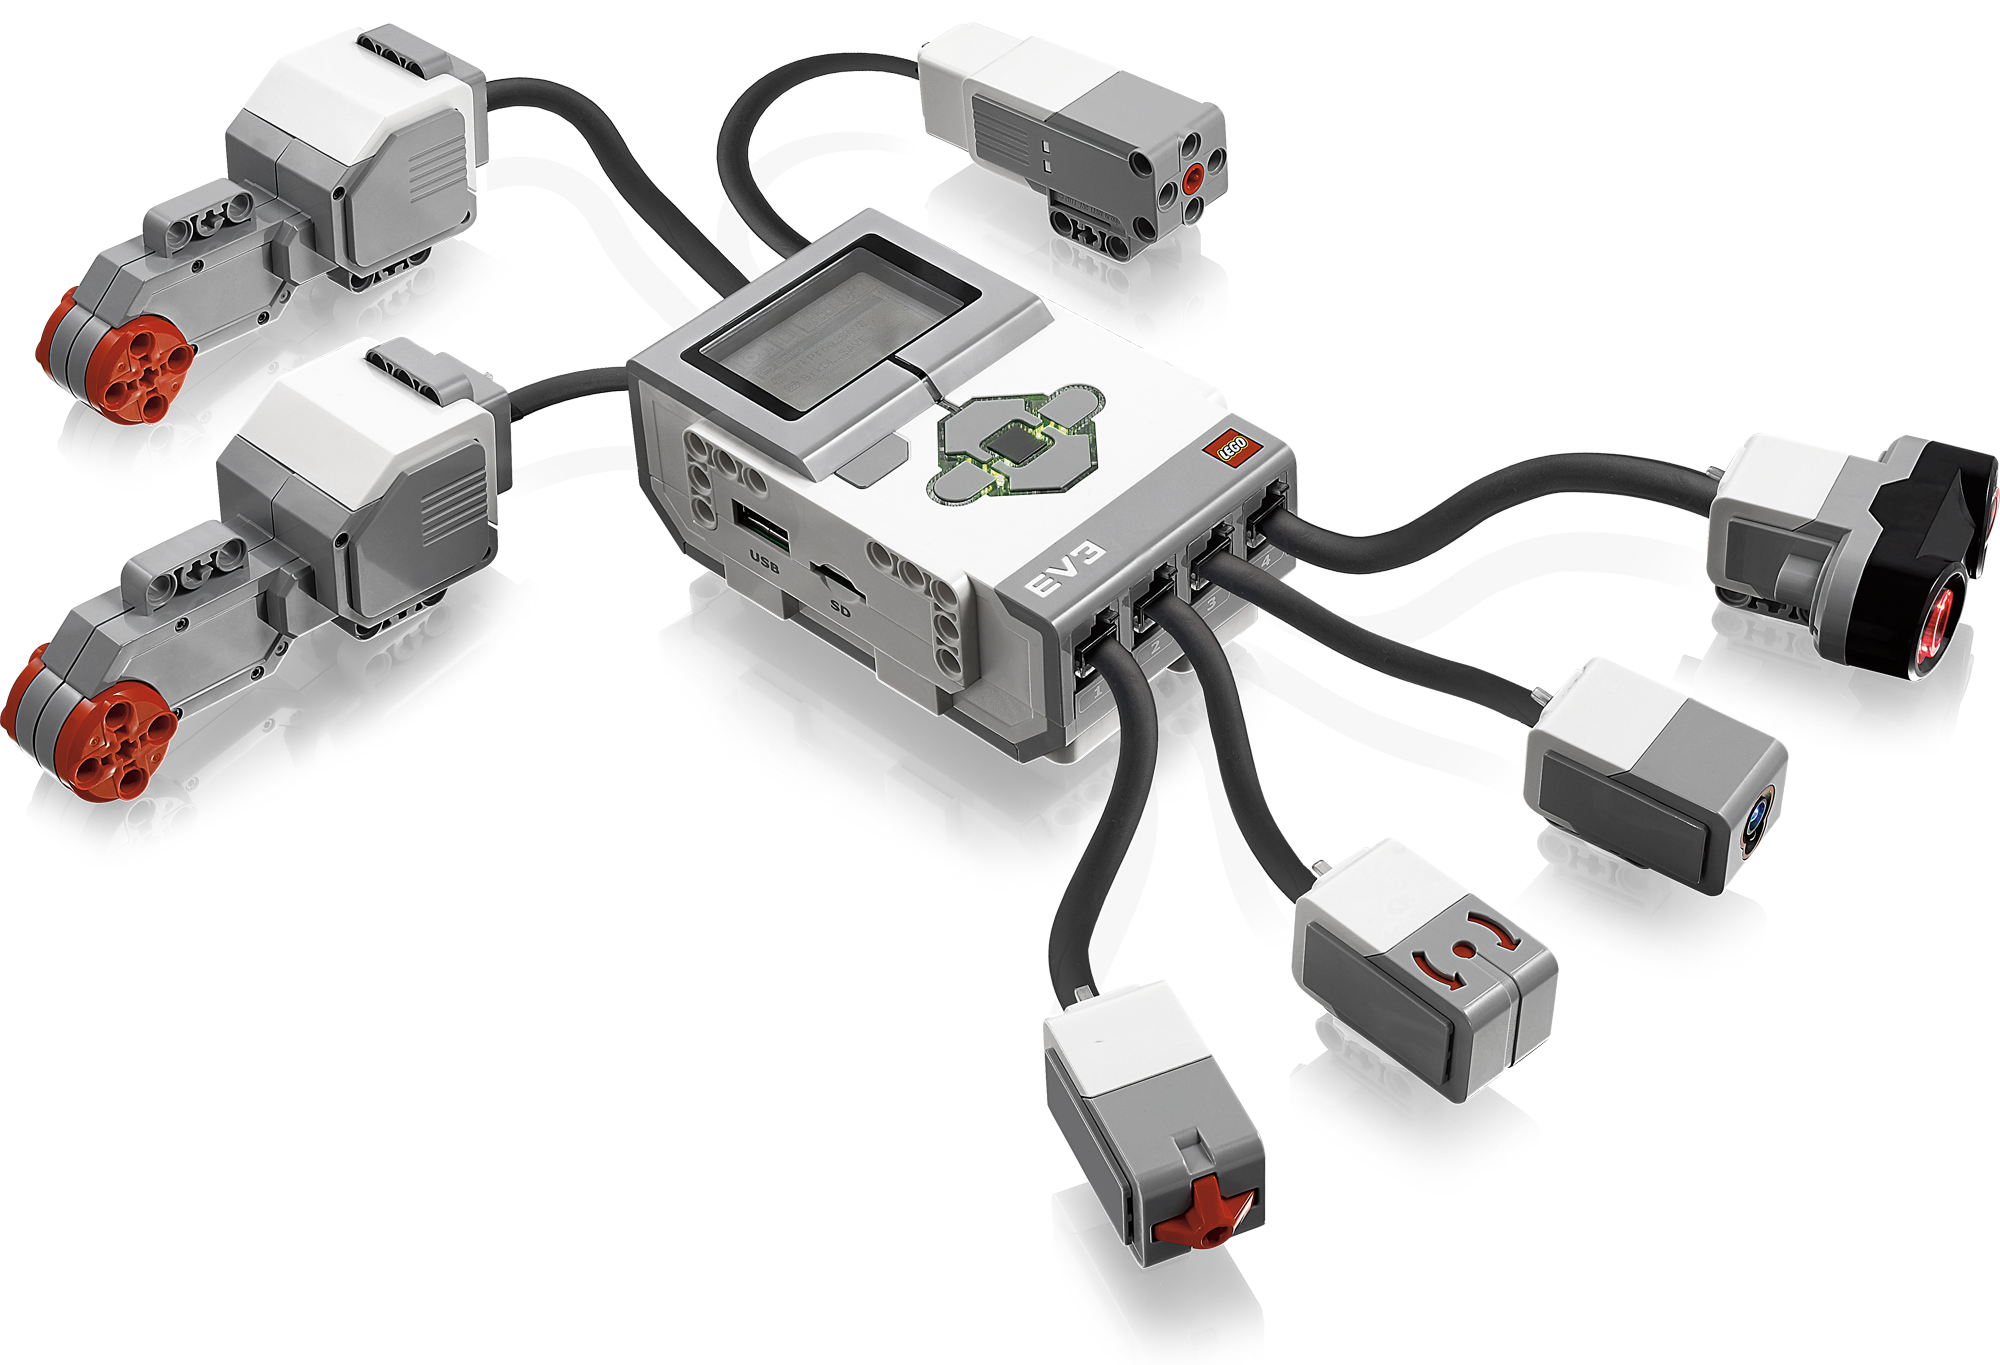
\includegraphics[width=0.90\textwidth]{images/technische_grundlagen/EV3-Overview.png}
	\caption[Zentrale Komponenten des EV3-Systems]{Zentrale Komponenten des EV3-Systems}
	\label{fig:<Sprungmakre>}
\end{figure}
\newline
Neben den elektronischen Komponeten gehören auch nicht elektronische Teile wie Verbindungsstücke, Balken und Zahnräder 
wie sie aus gängigen \LE{} Produkten bekannt sind, zum EV3-System. Sie bilden die strukturelle und meschanische Grundlage 
der Roboter.
\medskip
\newline
Im Folgenden wird auf die elektronischen Komponenten des EV3-Systems näher eingegangen.
dieses Projekt eine deutlich größere Relevanzu aufweisen.
\subsubsection{Der EV3-Stein (Steuereinheit)}
% Farbe die angibt welchen Status der folgende Abschnitt hat:
\color{finishing}
% Eigentlicher Text:
Die zentrale Komponenten und das Gehirn des LEGO MINDSTORMS EV3-Systems ist die zentrale Steuereinheit kurz (EV3-)Stein oder auch Brick genannt. Bei ihm handelt
es sich um eine Computer welcher selbständig Programme ausführen kann. Dazu verfügt der EV3-Stein über 
ein Linux Betriebssystem und eine spezielle Firmware, die wie die auszuführenden Programme auf einem Flash-Speicher liegen \cite[vgl.][21]{Scholz.DasEV3}. \\
Zur Kommunikation mit dem PC verfügt der EV3-Stein über eine USB- sowie Bluetooth-Schnittstelle. Neben der 
Kommunikation zu einem Computer kann die USB-Schnittstelle auch für den Zusammenschluss mit einem weiteren EV3-Stein (genannt Daisy Chain) 
genutzt werden \cite[vgl.][Seite 21]{Scholz.DasEV3}.  \\
Für den Anschluss von Motoren und Sensoren verfügt der EV3-Stein über 8 Ports, an welche die anderen System-Komponenten müber Kabel mit RJ12-Steckern angeschlossen werden. 4 der Ports dienen für den Anschluss von
Motoren, die restlichen 4 Ports für die Abfrage von Sensorwerte \cite[vgl.][21]{Scholz.DasEV3}.  \\
Der EV3-Stein besitzt an der Vorderseite ein LCD-Display zur Anzeige von Texten und Grafiken sowie  
6 Knöpfe für die Bedienung durch den Benutzer. Display und Knöpfe dienen zur Bedienung der Firmware sowie zur Tätigung von Einstellungen, können aber ebenso durch Programmen angesprochen und ausgewertet werden
Start
Mein Kanal
Trends
Abos
BIBLIOTHEK
\cite[vgl.][21]{Scholz.DasEV3}. 
\smallskip
\newline
Die folgende Auflistung zeigt einige Leistungsmerkmale des EV3-Steins \citep[vgl.][Seite 23 f., Seite 32]{Scholz.DasEV3, Schobel.RobertaEV3Programmieren}.
\begin{itemize}
	\item{Prozessor:} ARM9 32Bit, 300 MHz, 16 MB Flash 64MB RAM
	\item{Betriebssystem:} Linux
	\item{Sensoranschlüsse:} 4x, Analog / Digital bis zu 460,8 Kbit/s
	\item{USB-Schnittstellen:} 2x, für Kommunikation zum PC, Daisy Chain, WiFi-Stick, USB-Speichermedium
	\item{SD-Karten-Lesegerät:} 1x, für MicroSD-Karte bis 32 GB
	\item{User-Interface:} 6 Knöpfe inkl. Beleuchtung
	\item{Display:} LCD Matrix, monochrom, 178 x 128 Pixel
	\item{Kommunikation:} Bluetooth v2.1, USB 2.0 (Kommunikation zum PC), USB 1.1 (Daisy Chain)
\end{itemize}
\subsubsection{Motoren}
% Farbe die angibt welchen Status der folgende Abschnitt hat:
\color{finishing}
% Eigentlicher Text:
Das EV3-System verfügt über zwei unterschiedliche Motoren, einen großen Motor und einen mittleren Motor. 
Bei beiden handelt es sich um Servormotoren mit integriertem Rotationssensor, welche von außen angesteuert und abgefragt werden können \cite[vgl.][92]{Schobel.RobertaEV3Programmieren}. Die Motoren lassen sich sehr exakt steuern und ermöglichen so einen synchronen Betrieb mehrerer Motoren \cite[vgl.][Seite 29 f.]{Scholz.DasEV3}.
\smallskip
\newline
Die folgende Tabelle zeigt die wichtigsten Eigenschaften der beiden Motoren.
\begin{table}[ht]
	\begin{tabular}{|p{4,5cm}|p{4,0cm}|p{4,0cm}|} \hline
		Eigenschaft / Motortyp		                & Großer Motor         & Mittlerer Motor    \\ \hline
		Winkelgenauigkeit       & 1 $^\circ$           & 1 $^\circ$         \\ \hline
		Umdrehungen    			& 160 bis 170 U/min    & 240 bis 250 U/min  \\ \hline 
		Drehmoment Rotation		& 20 Ncm               & 8 Ncm    			\\ \hline  
		Drehmoment Stillstand 	& 40 Ncm               & 12 Ncm    			\\ \hline  
		Gewicht    				& 76g                  & 36g   		 		\\ \hline
	\end{tabular}
	\centering
	\caption[Eigenschaften der EV3-Motortypen]{Eigenschaften der EV3-Motoren}
\end{table}
\subsubsection{Sensoren}
% Farbe die angibt welchen Status der folgende Abschnitt hat:
\color{finishing}
% Eigentlicher Text:
Zum EV3-System gehören eine Reihe von verschiedenen Sensoren die es den Robotern ermöglichen Informationen über ihre Umwelt zu sammeln sowie ihre Eigenbewegungen zu erfassen. Im folgenden Abschnitt werden die wichtigsten Sensoren mit ihren Leistungsmerkmalen beschrieben.
\paragraph{Farbsensor}
% Farbe die angibt welchen Status der folgende Abschnitt hat:
\color{finishing}
% Eigentlicher Text:
Der Frabsensor ist ein digitaler Sensor der dazu dient die Lichtintensität sowie verschiedener Farben zu erkennen. Der Sensor kann sowohl
aktiv als auch passiv betrieben werden und verfügt dafür über vier unterschiedliche Betriebsmodi  \cite[vgl.][101]{Schobel.RobertaEV3Programmieren}:
\begin{itemize}
	\item{Farbmodus (passiv)} - In diesem Modus erkennt der Sensor 7 verschiedenen Farben.
	\item{RGB-Modus (aktiv)} - In diesem Modus sendet der Sensor nacheinander rotes, grünes und balues Licht aus, je nachdem zu welchem Anteil ein Gegenstand die einzelnen Farben reflektiert wird die Frabe des Gegenstands ermittelt.
	\item{Rotlicht-Modus (aktiv)} - Bei diesem Modus wird Rotlicht ausgesendet und die Intensität des reflektierten Lichts gemessen.
	\item{Umgebungslicht-Modus (passiv)} - Bei diesem Modus wird die Intesnsität des in das Sensorfenster eindringende Umgebungslichts gemessen.
\end{itemize}
\smallskip
Eigenschaften:
\begin{itemize}
	\item{Erkennung der Farben:} keine Farbe, Schwarz, Blau, Grün, Gelb, Rot, Weiß, Barun
	\item{Abtastrate:} 1.000 Hz
	\item{Entfrenung:} 15 bis 50 mm
\end{itemize}
Durch diesen Sensor wird es beispielsweise möglich den Roboter einer frabigen Linie auf dem Boden zu folgen.
\paragraph{Ultraschallsensor}
% Farbe die angibt welchen Status der folgende Abschnitt hat:
\color{finishing}
% Eigentlicher Text:
Diese aktive Sensor verwendet für den Menschen unhörbaren Ultraschall um die Entfernung von Objekten zu ermitteln.
Der Sensor emmitiert dazu Untraschall und misst die Laufzeit der Schallwellen, wenn diese von einem Objekt reflektiert
werden, aus der Laufzeit kann dann die Entfernung ermittelt werden.
Der Senors verfügt über zwei unterschiedliche Betriebsmodi \cite[vgl.][32 f.]{Scholz.DasEV3}:
\begin{itemize}
	\item{Messen} - In diesem Modus sendet der Sensor Ultraschall aus um die Entfernung von Objekten zu ermitteln.
	\item{Scannen} - In diesem passiven Modus emittiert der Sensor selbst keinen Untraschall, sondern er reagiert auf >>fremden<< Ultraschall und kann so einen anderen aktiven Ultraschallsensor erkennen.
\end{itemize}
\smallskip
Eigenschaften:
\begin{itemize}
	\item{Genauigkeit: +/- 1 cm}
	\item{Messbereich: 3 cm bis 250 cm}
\end{itemize}
\paragraph{Berührungssensor}
% Farbe die angibt welchen Status der folgende Abschnitt hat:
\color{finishing}
% Eigentlicher Text:
Der Berührungssensor ist ein einfacher mechanischer Sensor. Wird der Knopf am Ende des Senors gedrückt wird dies
registriert. Trotz der Einfachheit dieses Sensors ist dieser dennoch sehr nützlich, da er beispielsweise die
Kollision des Roboters mit einem Hindernis erkennen kann \cite[vgl.][33]{Scholz.DasEV3}.
\paragraph{Kreiselsensor (Gyroskop)}
% Farbe die angibt welchen Status der folgende Abschnitt hat:
\color{finishing}
% Eigentlicher Text:
Der Kreiselsensor ermöglicht es Drehbewegungen um eine Achse über Rotationsgeschwindigkeit und Drehwinkel zu 
messen. Dadurch wird es möglich die Eigenbewegung des Roboters oder einer Roboterkomponente zu registrieren 
\cite[vgl.][33]{Scholz.DasEV3}.
\medskip
\newline
Eigenschaften:
\begin{itemize}
	\item{Genauigkeit: +/- 3$^\circ$ (bei einer 90$^\circ$ Drehung)}
	\item{Geschwindigkeit: maximal 440 Grad/Sekunde}
	\item{Abtastrate: 1.000 Hz}
\end{itemize}
\paragraph{Rotationssensor (Integiert)}
% Farbe die angibt welchen Status der folgende Abschnitt hat:
\color{finishing}
% Eigentlicher Text:
Wie bereits im Abschnitt X.X dargelegt verfügen die beiden Motortypen über initgrierte Rotationssensoren die es
ermöglichen, die Umdrehungen der Motoren auszulesen. Durch diese Sensoren ist es möglich durch Odometrie 
Rückschlüsse über die Bewegung bzw. Position des Roboters zu schließen.
\medskip
\newline
Eigenschaften:
\begin{itemize}
	\item{Genauigkeit: 1$^\circ$ }
	\item{Umdrehungen: Motorabhängig}
\end{itemize}
\bigskip
Neben den hier vorgestellten Sensoren existiert noch ein Infrarotsensor, welcher in Verbindung mit einer Infrarotfernsteruerung dazu dient einen EV3-Roboter fernzusteuern.
%### Subsubsektion über XXX ################################################################################################################
\subsubsection{Programmierung}
% Farbe die angibt welchen Status der folgende Abschnitt hat:
\color{process}
% Eigentlicher Text:
Für die Programmierung der \LM{} Produkte gibt es eine Reihe unterschiedlicher Programmiersprachen und -umgebungen. Die hauseigene \LE{}-Software zur Programmierung des EV3 richtet sich an Einsteiger. Sie ermöglicht es über eine grafische Oberfläche via vorgefertigter Programmabläufe welche durch grafische Blöcke repräsentiert werden den EV3 zu programmieren.\footnote{\citep[vgl.][25 f.]{Schobel.RobertaEV3Programmieren}\label{Roberta25psq}} \\
%cite[vgl.][25\psq]{Roberta}.
Die Abbildung X.X gibt einen Überblick über verschiedene für den EV3 verfügbare Programmiersprechen sowie ihre Vor- und Nachteile.
\paragraph{leJOS}
Das LEGO Java Operating System abgekürzt leJOS ist ein Framework, das es ermöglicht den EV3 mit der Programmiersprache Java zu programmieren. Das leJOS-Projekt wurde 1999 gegründet und sämtliche Komponenten (wie auch Java) sind kostenlos verfügbar \cite[vgl.][21 f.]{Schobel.RobertaEV3Programmieren}. \\
leJOS bietet eine schlanke Java Virtual Machine (JVM) für den EV3-Stein sowie eine Klassenbibliothek mit welcher die Komponenten des EV3 (Motoren, Sensoren etc.) angesprochen werden können. Installiert wird leJOS auf einer bootbaren microSD-Karte und kann anschließend davon gestartet werden, ohne die auf dem EV3 vorhandene LEGO-Software zu löschen oder zu verändern \cite[vgl.][23 f.]{Schobel.RobertaEV3Programmieren}. \\
Durch leJOS ist es möglich den EV3 mit Hilfe der Hochsprache Java zu programmieren womit eine mächtige
Programmiersprache zur Verfügung steht und die Vorteile der Objektorientierung für den EV3 genutzt werden können.
\begin{table}[ht]
	\begin{tabular}{|p{4,5cm}|p{2,0cm}|p{2,0cm}|p{2,0cm}|p{2,0cm}|} \hline
		Eigenschaft / Programmiersprache  & leJOS      & EV3-Software  & RobotC  & NEPO       \\ \hline
		Installation                      & +          & ++            & +       & +++        \\ \hline
		Handhabung    		           	  & +          & ++            & +       & ++         \\ \hline
		Kosten                            & kostenlos  & kostenlos     & 49\$    & kostenlos  \\ \hline
		Einstieg 	                      & 0          & ++            & +       & +++        \\ \hline  
		Funktionsumfang    				  & ++         & +             & ++      & ++         \\ \hline
	\end{tabular}
	\centering
	\newline
	0 = neutral; + = gut; ++ = sehr gut; +++ = hervorragend
	\caption[Eigenschaften der EV3-Motortypen]{Eigenschaften der EV3-Motoren}
\end{table}
leJOS bietet eine umfangreiche Klassenbibliothek sowie gut dokumentierte API was unter anderem die
Integration von weiteren Sensoren etc. erleichter \cite[vgl.][23 f.]{Schobel.RobertaEV3Programmieren}.
Im folgenden sind einige Features die leJOS bietet aufgelistet:
\begin{itemize}
	\item{Objektorientierte Programmierung mit Java}
	\item{Die meisten Klassen der Pakete \code{java.lang}, \code{java.util} und \code{java.io}}
	\item{Rekursion}
	\item{Synchronisation}
	\item{Multithreading}
	\item{Exceptions}
	\item{Vollständige Bluetooth unterstützung}
	\item{Unfangreiche Klassenbibliothek zum Steuern und Auslesen der EV3-Komponeten}
	\item{High-Level-Robotik-Tasks (Navigation, Localization etc.)}
\end{itemize}

\newpage
\color{finishing}
\subsection{\gls{app} Entwicklung} %Simon ca. 8

\begin{wrapfigure}{r}{0.45\textwidth}
	\begin{center}
		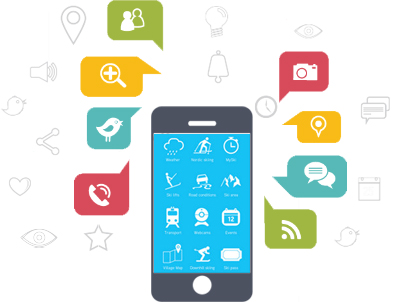
\includegraphics[width=0.4\textwidth]{images/technische_grundlagen/App-Development.jpg}
	\end{center}
	\caption{App Entwicklung \cite{Nethority.Web&App}}	
	\label{fig:appentwicklung}
\end{wrapfigure}

Eine \gls{app} ist ein ausführbares Programm für mobile Geräte, wie Smartphones oder Tablets. Um eine \gls{app} für ein mobiles Gerät zu entwickeln, müssen wie für andere Anwendungen im Voraus Anforderungen definiert werden, die diese erfüllen soll. Je nach festgelegten Anforderungen, die an das System gestellt werden, besteht eine bestimmte Anzahl von Möglichkeiten der Entwicklung. Allgemein kennt die \gls{app} Entwicklung drei verschiedene Arten, die native, web und hybride Entwicklung, siehe \eqref{native}, \eqref{web} und \eqref{hybride}. Dabei werden verschiedene \glspl{framework} verwendet, um mit unterschiedlichsten Programmiersprachen den Aufbau der Logik zu beschreiben. Eine App besteht immer aus zwei Teile, dem \gls{ui}, das meist mit einer \gls{xml} ähnlichen Sprache beschrieben wird und dem Programmcode, der sich auf viele Klassen verteilt und die Funktionalitäten der \gls{app} beschreiben.

\subsubsection{Native \glspl{app}}\label{native}

In der Entwicklung von nativen \glspl{app} werden die direkten Ressourcen des Gerätes verwendet. Dazu gehört die Laufzeitumgebung des Betriebssystemes, Bibliotheken und Hardwareschnittstellen. Der Vorteil von einer nativen Entwicklung liegt hauptsächlich darin, dass diese für das Betriebssystem optimiert ist und die vorhandenen Schnittstellen genutzt werden können, um komplexe und rechenintensive Anwendungen zu ermöglichen.\footnote{\citep[vgl.][Unterschiede und Vergleich native Apps vs. Web Apps]{DanielWurstl.Unterschiedeund}\label{note1}}\\
Vertreter diese Entwicklung finden sich für verschiedene Betriebssysteme. Der populärste unter ihnen ist bei weitem Android mit einer nativen Java Entwicklung über Android Studio von Google. Sie besitzt aktuellen den höchsten Marktanteil und eine entsprechende Popularität unter Entwickler und Nutzer.

\subsubsection{Web \glspl{app}}\label{web}

Die Entwicklung von web \glspl{app} arbeitet mit systemübergreifenden Ressourcen und greift auf gängige Webtechnologien, wie \gls{html}, \gls{css} und \gls{javascript} zurück. Die \gls{app} wird hierbei nicht wie normale Anwendungen direkt auf dem System des Gerätes ausgeführt, sondern kommt in dessen Browser zur Ausführung. Der Vorteil hierbei ist vor allem, dass diese Art von \gls{app} auf allen Betriebssystemen lauffähig ist und direkt über das Internet veröffentlicht und aktualisiert werden kann, jedoch wird eine stabile Internetverbindung vorausgesetzt.\footref{note1}\\
Von dieser Entwicklung finden sich viele Vertreter mit der Unterstützung diverser \glspl{framework}. Das populärste unter ihnen ist aktuell AngularJS von Google, was auf \gls{javascript} basiert. In Kombination mit anderen Webtechnologien, wie \gls{html} und \gls{css} lassen sich perfomante web \glspl{app} entwickeln.

\subsubsection{Hybride \glspl{app}}\label{hybride}

Die Entwicklung von hybride \glspl{app} vereinigt die beiden Entwicklungen von native und web. Sie besteht dabei aus einem nativen Rahmen, in der eine web \gls{app} zur Ausführung kommt, diese besitzt entsprechende Zugriffsrechte auf Hardwareschnittstellen, um diese mit \glspl{api} anzusprechen.\footnote{\citep[vgl.][Native App, Web App und Hybrid App im Überblick]{PetraRiepe.NativeApp}\label{note2}}\\
Diese Entwicklung ist aktuell noch sehr jung, jedoch stechen hier bereits verschiedene Vertreter hervor. Der populärste unter ihnen ist Ionic von Drifty, welches auf Apache Cordova als Basis zurückgreift. In Kombination mit AngularJS, \gls{typescript} und anderen Webtechnologien lässt sich die web \gls{app} entwickeln und auf einem beliebigen Gerät unter einem nativen Browser ausführen. Es unterstützt dabei verschiedenste Betriebssystem, wie Android, iOS und Windows. Diese Entwicklungen können dabei meist nicht nur mobil, sondern unter anderem auf weiteren Systemen, wie stationäre bereitgestellt werden.

\subsubsection{Plattformübergreifende Entwicklung}

Um die Entwicklung von \glspl{app} einfach zu halten, verwenden immer mehr Entwickler die Form der plattformübergreifenden Entwicklung. Dadurch lässt sich die \gls{app} unabhängig des Betriebssystems entwickeln und kann somit eine größere Menge von Nutzern erreichen. Diese Entwicklung greift dabei meist auf plattformübergreifende Konzepte, wie eine native Laufzeitumgebung, oder Browser zurück, um darin die \gls{app} auszuführen. Der große Vorteil in dieser Entwicklung, liegt in der Wiederverwendbarkeit des Quellcodes und der verbesserten Wartbarkeit, da hier lediglich ein Projekt gewartet werden muss und der Quellcode für viele Betriebssysteme übernommen werden kann. Zur plattformübergreifenden Entwicklung wurden die letzten Jahre viele Ansätze mit verschiedenen \glspl{framework} entwickelt. Beispiele hierfür sind Ionic, Unity, Qt oder Xamarin.\\
\newpage

\subsubsection{Xamarin}

\begin{wrapfigure}{r}{0.3\textwidth}
	\begin{center}
		
\includegraphics[width=0.25\textwidth]{images/technische_grundlagen/xamarin.png}
	\end{center}
	\caption{Xamarin \cite{Xamarin}}
	\label{fig:xamarin}
\end{wrapfigure}

Xamarin ist ein \gls{framework} zur Entwicklung von nativen plattformübergreifenden Apps, welches auf Mono basiert, siehe \eqref{mono}. Um nativen Quellcode auf den verschiedenen Systemen auszuführen, setzt Xamarin auf verschiedene Softwarekomponenten, um aus einem mit .NET entwickelten Projekt nativen Quellcode zu erzeugen.\\
Für iOS Systeme verwendet Xamarin den \gls{aot} Compiler, um aus einem Xamarin.iOS Projekt \gls{arm} Maschinencode zur erzeugen, der entsprechend schnell auf dem System ausgeführt werden kann.\footnote{\citep[vgl.][Introduction to Mobile Development - Xamarin]{Xamarin.Introductionto}\label{note3}} Bei Android hingegen wird der Quellcode in \gls{il} übersetzt, welches \gls{jit} nutzt um zur Laufzeit Maschinencode für das entsprechende Gerät zu erzeugen.\footref{note3} Dazu nutzt Xamarin Softwarekomponenten, während der Laufzeit, um bestimmte Prozesse, wie Speicherverwaltung und Plattformoperationen. Zur Entwicklung bringt Xamarin eine große Bandbreite von Funktionalitäten für den Entwickler, wie Bibliotheken, eine Test Cloud, sowie Unterstützung von nativen Bibliotheken, wie für \gls{java} oder \gls{objectivc}. Xamarin bietet Unterstützung für diverse Betriebssysteme, wie zum Beispiel Android, iOS, Windows und Windows Phone. Um mit Xamarin zu entwickeln, gibt es aktuell verschiedene Möglichkeiten mit Unterstützung auf unterschiedlichen Betriebssystemen. Einerseits kann mit Xamarin Studio auf einem OSX System, oder mit Visual Studio auf Windows und Linux entwickelt werden.\\
Wie viele andere \glspl{framework}, bietet auch Xamarin verschiedene nützliche \glspl{template}, die jeweils andere Nutzen besitzen. Diese bauen dabei auf zwei Hauptkomponenten von Bibliotheken, einerseits Shared Projects und Protable Class Libraries.

\begin{wrapfigure}{r}{0.55\textwidth}
	\begin{center}
		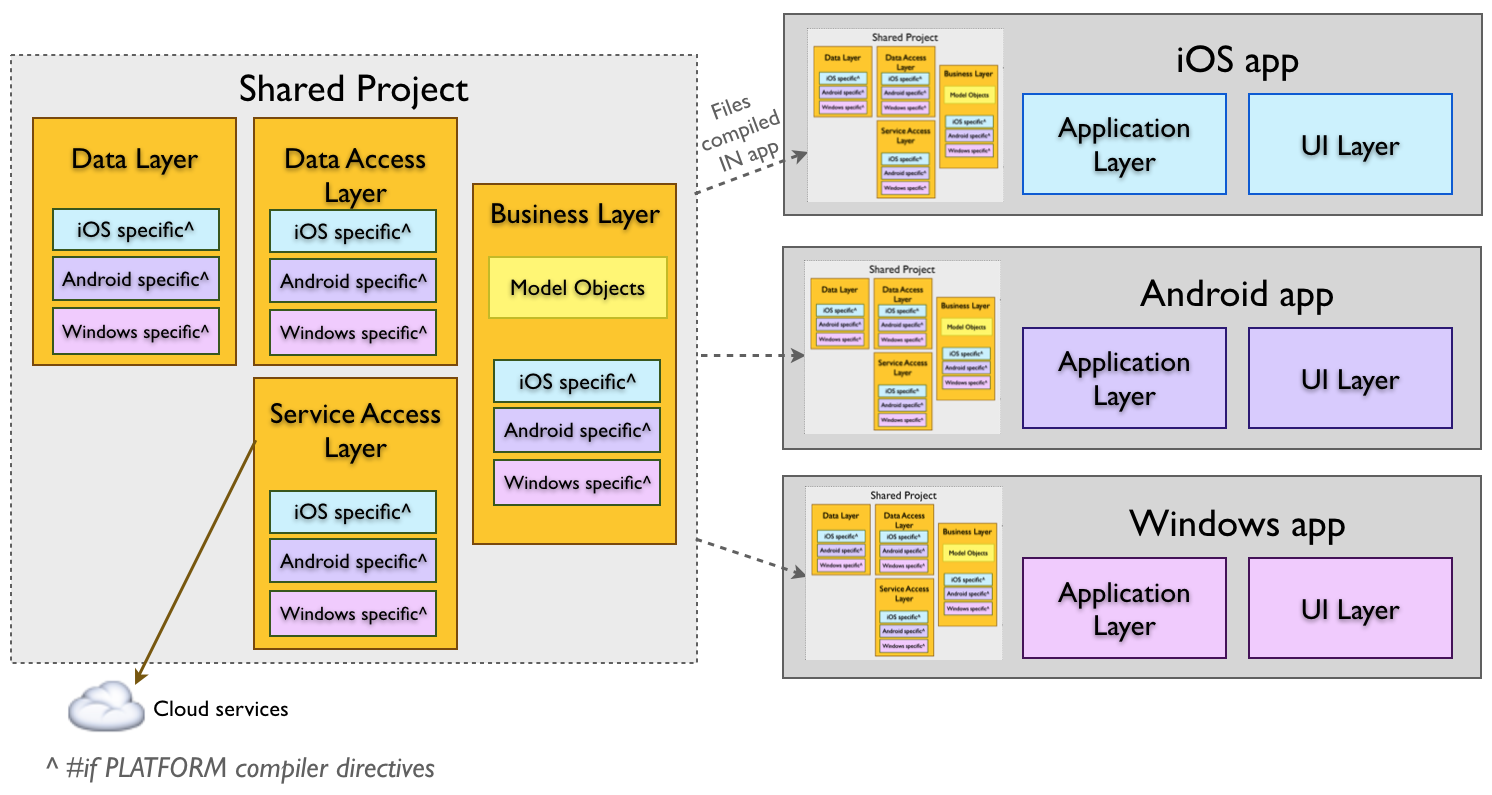
\includegraphics[width=0.5\textwidth]{images/technische_grundlagen/SharedAssetProject.png}
	\end{center}
	\caption{Shared Project \cite{Xamarin.SharedProjects}}
	\label{fig:shared}
\end{wrapfigure}

\paragraph{Shared Projects}

ermöglichen dem Entwickler Quellcode für verschiedene Plattformen zu entwickeln, wobei die plattformspezifischen Projekte das entsprechende shared Project referenzieren. Somit besitzt diese Projektart keinen direkten Output, sondern kopiert den Quellcode in das zu entsprechend bauende Projekt, siehe Abbildung \eqref{fig:shared}.\footnote{\citep[vgl.][Shared Projects - Xamarin]{Xamarin.SharedProjects}\label{note4}} Der Hauptunterschied zu Standardprojekten liegt vor allem darin, dass ein shared Project keine Abhängigkeiten haben darf und daher lediglich als Referenz für andere Projekte dienen kann.

\begin{wrapfigure}{r}{0.55\textwidth}
	\begin{center}
		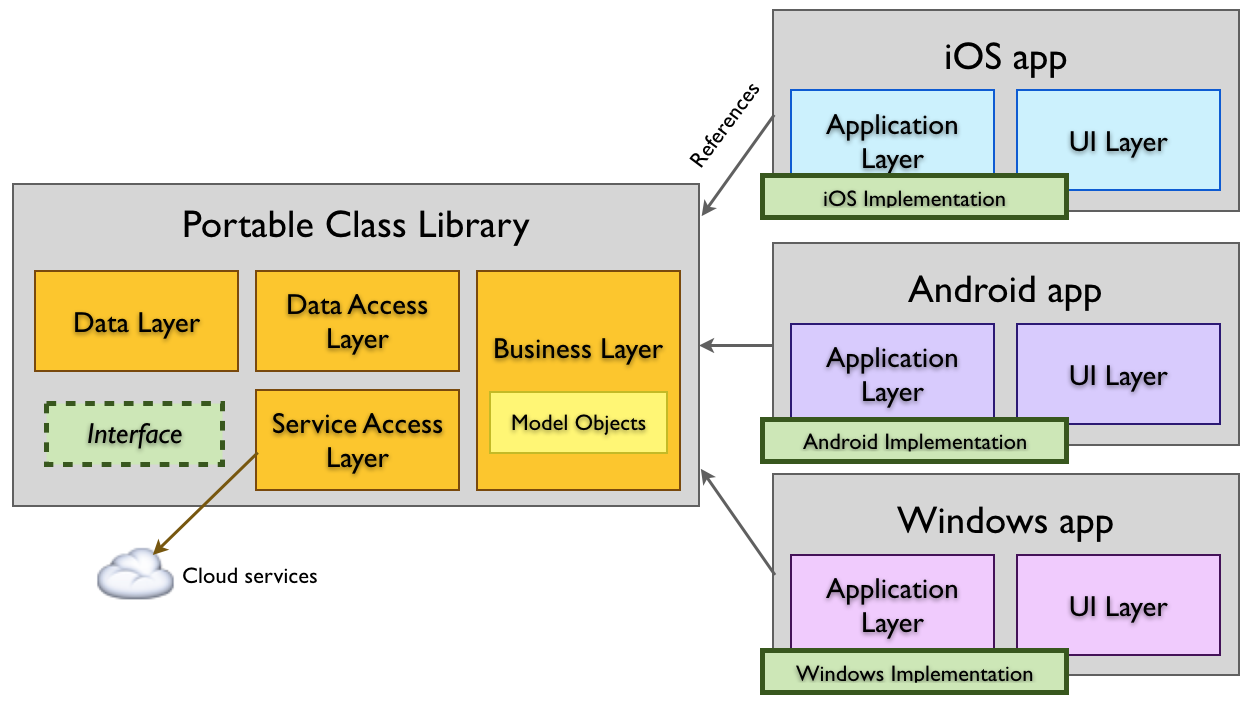
\includegraphics[width=0.5\textwidth]{images/technische_grundlagen/PortableClassLibrary.png}
	\end{center}
	\caption{Portable Class Library \cite{Xamarin.PortableClass}}
	\label{fig:portable}
\end{wrapfigure}

\paragraph{Protable Class Libraries}

ermöglichen dem Entwickler die Implementierung von plattformübergreifende Bibliotheken, aus denen \glspl{dll} erzeugt werden können. Das Besondere an Portable Class Libraries ist dabei, dass die Plattformen spezifisch ausgewählt werden können, wobei auf die Unterstützung verschiedener Betriebssysteme zu achten ist, siehe Abbildung \eqref{fig:pcl_support}.\footnote{\citep[vgl.][Introduction to Portable Class Libraries - Xamarin]{Xamarin.PortableClass}\label{note5}} Eine Portable Class Library besitzt darüber hinaus verschiedene Vor- bzw. Nachteile, die für oder Gegen ihre Nutzung sprechen.\\

\begin{wrapfigure}{r}{0.55\textwidth}
	\begin{center}
		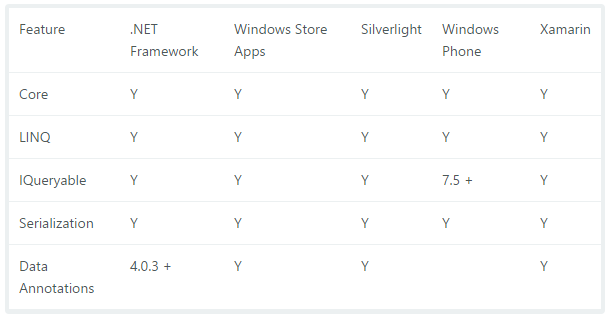
\includegraphics[width=0.5\textwidth]{images/technische_grundlagen/pclSupport.png}
	\end{center}
	\caption{Unterstützung Portable Class Library \cite{Xamarin.PortableClass}}
	\label{fig:pcl_support}
\end{wrapfigure}

\noindent
Vorteile:
\begin{itemize}
	\item Implementierung von zentralem Quellcode
	\item Einfaches Refactoring
	\item Referenzierung von Anwendungen
\end{itemize}
\noindent
Nachteile:
\begin{itemize}
	\item Keine Referenzierung von Plattform spezifischem Quellcode
	\item Keine Standardbibliotheken vorhanden
\end{itemize}

\newpage
\subsubsection{Mono}\label{mono}

\begin{wrapfigure}{r}{0.3\textwidth}
	\begin{center}
		
\includegraphics[width=0.25\textwidth]{images/technische_grundlagen/mono.png}
	\end{center}
	\caption{Mono \cite{Mono.MonoProject}}
	\label{fig:mono}
\end{wrapfigure}

Mono ist ein opensource Framework, das auf dem .NET Framework von Microsoft basiert. Die Implementierung von Mono greift dabei auf die Standards von .NET für die Programmiersprache \gls{csharp}, sowie die \gls{cli} zurück.\footnote{\citep[vgl.][About Mono]{MonoProject.AboutMono}\label{note6}} Dies ermöglicht Entwicklern die Erstellung von plattformübergreifenden Anwendungen, welche mittels einer zur Verfügung gestellten Laufzeitumgebung auf verschiedenen Systemen ausgeführt werden können.\\
Um Anwendungen auf verschieden Systemen auszuführen, nutzt Mono verschiedene Komponenten. Dazu gehört an vorderster Stelle ein Compiler, um den erstellten Quellcode in die jeweilige Maschinensprache zu übersetzen. Die Übersetzung findet dabei in Kooperation der Mono Runtime statt, die die entsprechende Infrastruktur zur Ausführung der Anwendung bereitstellt. Für eine effiziente Entwicklung stellt Mono zwei Bibliotheken zur Verfügung, einerseits die .NET Class Library, die die Grundelemente von .NET enthält, sowie die Mono Class Library mit zusätzlichen Funktionen für plattformübergreifende Anwendungen.\\
Für die Nutzung von Mono stehen verschiedene Vorteile im Vergleich zu anderen Framework. Der Hauptgrund für die Nutzung liegt vor allem in der Popularität von .NET, da dies auf den meisten Computern zur Verfügung steht, oder installiert werden kann. Ein großer Nutzen stellt die High-Level Programmierung dar, die eine Implementierung mit einer Laufzeitumgebung ermöglicht, die Funktionen wie Speicherverwaltung selbst organisiert. Durch Verwendung der \gls{clr} kann der Entwickler seine übliche Programmiersprache verwenden und ist unhabhängig vom bestehenden System.

\subsubsection{.NET Framework}\label{net}

Das .NET Framework dient zur Entwicklung sowie Ausführung von Anwendungen, die mit Programmiersprachen implementiert werden und auf den Standards von .NET basieren. Es besteht aus verschiedenen Komponenten, wobei der Kern des Frameworks in der \gls{clr} liegt.\footnote{\citep[vgl.][Overview of the .NET Framework]{Microsoft.Overviewof}\label{note7}} Diese ist verantwortlich für die Laufzeitumgebung und entsprechend für die Ausführung der Anwendungen, indem es die bereitgestellten Ressourcen des Systems nutzt.\\
\begin{wrapfigure}{r}{0.45\textwidth}
	\begin{center}
		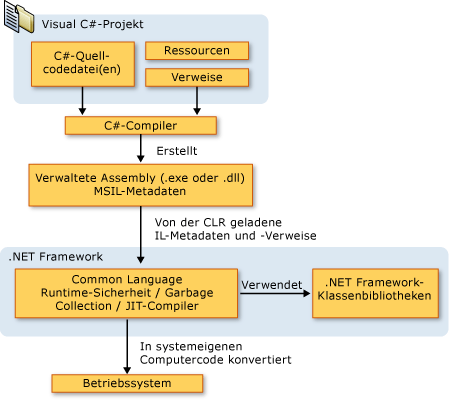
\includegraphics[width=0.4\textwidth]{images/technische_grundlagen/net_aufbau.jpeg}
	\end{center}
	\caption{.NET Framework Ausführung}
	\label{fig:net}
\end{wrapfigure}

\noindent
Die \gls{clr} führt zur Laufzeit je nach System verschiedene Aktionen aus, um die entsprechende Anwendung auszuführen. Der allgemeine Ablauf ist dabei folgender. Der Quellcode wird in die \gls{clr} geladen und nach Sicherheitsanforderungen entsprechend des Systems überprüft.\footref{note7} Anschließend wird er durch eine \gls{jit} Kompilierung in einen \gls{il} Quellcode konvertiert, um diesen nativ auf dem System ausführen zu können.\footref{note7} Der \gls{il} Quellcode setzt dabei auf die gesetzten Standards der \gls{cli} auf, die eine sprach- und plattformunabhängige Entwicklung von Anwendungen ermöglicht.\footref{note7}\\
Das .NET Framework bietet zusätzlich zur unabhängigen Entwicklung verschiedene unterstützende Komponenten. Die wichtigste unter ihnen ist die .NET Class Library. Diese unterstützt den Entwickler mit einer Sammlung bereits implementierten Quellcode, wie Klassen und entsprechenden Zugang zu systemnahen Schnittstellen. Mit dem .NET Framework lässt sich eine große Bandbreite von Anwendungen entwickeln, von Konsolenanwendungen, grafischen Oberflächen, bis hin zu Webanwendungen.\\

\begin{figure}[h]
	\centering
	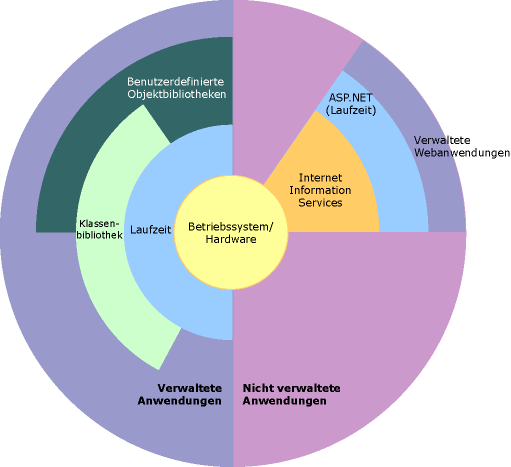
\includegraphics[width=0.65\textwidth]{images/technische_grundlagen/clr.png}
	\caption{Common Language Runtime}
	\label{fig:clr}
\end{figure}

\color{process}

\subsection{TCP-Kommunikation}
Das Transmission Control Protocol (TCP) ist ein Transportprotokoll und ermöglicht eine Datenaustausch zwischen kommunizierenden Anwendungsinstanzen in einer Ende-zu-Ende-Beziehung zwischen. TCP ist als Transportprotokoll auf in der 4 Schicht des OSI-Modells angesiedelt und basiert auf dem Internetprotokoll (IP) mit dem zusammen es als Nahmensgeber der TCP/IP-Protokollfamilie (Internetprotokollfamilie) dient.
TCP ist ein offenes, frei verfügbares und weit verbreitetes Protokoll. Als Mitglied der Internetprotokollfamilie ist TCP neben UDP das Transportprotokoll, auf dem die meisten Anwendungen im Internet basieren [GD189].
\subsubsection{Gundlegendes}
Als verbindungsorientiertes Protokoll sorgt TCP für die Erzeugung und Erhaltung einer gesicherten 
Ende-zu-Ende-Verbindung zwischen zwei Anwendungsprozessen. TCP arbeitet paketvermittelt d.h. überträgt Daten Paketweise und ist ein zuverlässiges Protokoll.
Durch diese Eigenschaften stellt TCP sicher dass, Daten
\begin{itemize}
	\item{nicht verloren gehen}
	\item{nicht verändert werden}
	\item{nicht dupliziert werden}
	\item{in der richtigen Reihenfolge eintreffen}
\end{itemize}
Zur Gewährleistung einer vollständingen Übertragung sowie der Integrität der gesendeten Daten nutzt TCP Prüfsummen,Bestätigungen, Zeitüberwachungs- und Nachrichtenwiederholungsmechanismen sowie Sequenznummern für die Reihenfolgeüberwachung und das Sliding Windows Prinzip zur Flusskontrolle [GD].
\newline
TCP nutzt prinzipiell folgende Protokollmechanismen:
\begin{itemize}
	\item{Drei-Wege-Handshake-Verbindungsauf- und -abbau}
	\item{Positives, kumulatives Bestätigungsverfahren mit Timerüberwachung für jede Nachricht}
	\item{Implizites negatives Bestätigungsverfahren (NAK-Mechanismus): Bei drei ankommenden Duplikat-ACK-PDUs wird beim Sender das Fehlen des folgenden Segments angenommen. Ein sog. Fast-Retransmit-Mechanismus führt zur Neuübertragung des Segments, bevor der Timer abläuft.}
	\item{Pipelining}
	\item{Go-Back-N zur Übertragungswiederholung}
	\item{Fluss- und Staukontrolle}
\end{itemize}
\subsubsection{Nagle-Algorithmus}
Nagle-Algorithmus (RFC 896 und RFC 1122) ist ein Algorithmus der der Optimierung dient und der bei allen 
TCP-Implementierungen verwendet wird. Der versuchte Nagle-Algorithmus aus Optimierungsgründen zu verhindern, dass viele kleine Nachrichten gesendet werden, da dies schlecht für die Netzauslastung ist [GD198]. \newline
Dazu werden mehrere Nachrichten zusammengefasst und gebündelt versendent, dies geschieht nach folgendem Prinzip:
\begin{itemize}
	\item{Erhält der TCP-Endpunkt Daten vom Anwendungsprozess wird zunächst nur das erste Datenpaket gesendet und die restlichen Daten werden im Sendepuffer gesammelt.}
	\item{Danach werden weiteren Daten so lange im Sendepuffer gesammelt bis alle zuvor gesendeten Datenpakete vom Empfänger bestätigt wurden oder so viele Daten im Sendepuffer liegen das die eingstellte Segmentgröße erreicht ist und ein volles Datenpaket gesendet werden kann.}
\end{itemize}
Dieses Verfahren sorgt zwar für eine gute Netzauslastung da das Verhältnis von Nutzdaten zu Overhead (TCP-Header etc.) steigt jedoch ist dies allerdings nicht nicht für alle Anwendungsszenarien optimal da es die Latenz erhöt. Insbesondere bei Anwendungen die eine ummittelbare Antwort der Gegenstelle benötigen wie SSH- oder Telnet-Anwendung sorgt dies für Verzögerungen. In diesem Fall ist es besser den Nagle-Algorithmus auszuschalten. [GD198 f.]
\subsubsection{Kommunikationsablauf}
Da es sich bei TCP um ein verbindungsorientiertes Protokoll handelt gliedert sich die Kommunikation in die drei Phasen Verbindungsaufbau, Datenaustausch und Verbindungsabbau. Bevor Daten übertragen werden können muss die Verbindung durch den Verbindungsaufbau initiert und nach Beendinung der Datenbertragung
wieder abgebaut werden. 
\paragraph{Client \& Server}
Der Verbindungsaufbau einer Kommunikation erfolgt bei TCP nach dem Client-/Server-Paradigma, d.h. einer der Teilnehmern aggiert als Server und wartet auf einen Verbindungsaufbau durch den Client welchen der andere Teilnehmern darstellt. \newline
Nach dem Verbindungsauffbau haben die beiden Rollen jedoch keine Bedeutung mehr und die beide Teilnehmern
sind sowohl bei der Datenübertragung als auch beim Verbindungsabbau gleichberechtigt.
\paragraph{Verbindungsaufbau} \code{}
\newline
\smallskip
\begin{figure}[ht]
	\centering
	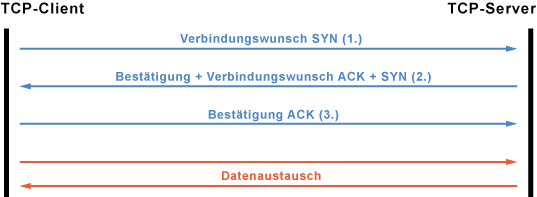
\includegraphics[width=0.8\textwidth]{images/Verbindungsaufbau.png}
	\caption[TCP Verbindungsaufbau]{TCP Verbindungsaufbau}
	\label{fig:<Sprungmakre>}
\end{figure}
Der Verbindungsaufbau bei TCP basiert auf dem Three-Way-Handshake. Dabei schickt der schickt der Client einen Verbindungswunsch (SYN) an den Server. Der Server bestätigt den Erhalt der Nachricht (ACK) und äußert seinerseits einen Verbindungswunsch (SYN) welchen der Client nach Erhalt der Nachricht bestätigt (ACK). Nach Abblauf dieses gegenseitigen Anfrage- und Bestätigugsvorgangs ist die Verbindung initiiert und der Datenaustausch zwischen den Teilnehmern kann beginnen [EK].
\paragraph{Datenaustausch}
\begin{figure}[ht]
	\centering
	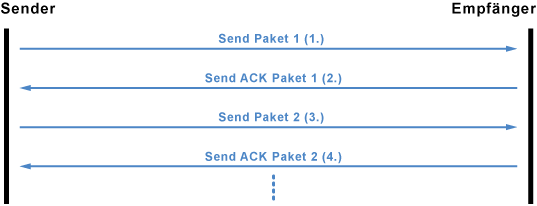
\includegraphics[width=0.8\textwidth]{images/Datenaustausch.png}
	\caption[TCP Datenaustausch]{TCP Datenaustausch}
	\label{fig:<Sprungmakre>}
\end{figure}
\paragraph{Verbindungsabbau}
\begin{figure}[ht]
	\centering
	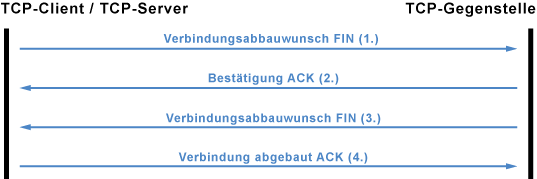
\includegraphics[width=0.8\textwidth]{images/Verbindungsabbau.png}
	\caption[TCP Verbindungsabbau]{TCP Verbindungsabbau}
	\label{fig:<Sprungmakre>}
\end{figure}
Nach Abschluss der Datenübertragung wird von einer Seite (egal von welcher) ein Verbindungsabbau initiiert. Dazu dient einen etwas modifizierten Drei-Wege-Handshake-Mechanismus. Jede der beiden Verbindungsrichtungen der Vollduplex-Verbindung wird abgebaut, d.h. beide Seiten bauen ihre „Senderichtung“ ab. Die initiierende Seite schickt zuerst einen Verbindungsabbauwunsch (FIN). Die Gegenstelle bestätigt den Erhalt der Nachricht (ACK) und schickt ebenfalls einen Verbindungsabbauwunsch (FIN) woraufhin sie von der Gegenstelle noch mitgeteilt bekommt, dass die Verbindung abgebaut ist (ACK).
\subsubsection{Socket-Programmierung}
Als Transportzugriffsschnittstelle für die TCP-basierte Kommunikation dient die Socket-Schnittstelle.
Obwohl es sich bei TCP ein paketvermitteltes Protokoll handlet der Anwendung eine Strom-orientierte Kommunikation, die Daten werden also von einem Anwendungsprozess Byte für Byte in einem Bytestrom geschrieben und TCP sorgt anschließend um den Aufbau von Segmenten, die dann übertragen werden. Andere Transportdienste erwarten ihre Daten in festen Blöcken [GD].

\newpage
\color{finishing}
\subsection{Schwarmverhalten}

Dieser Abschnitt beschäftigt sich mit dem Schwarmverhalten, welches mit Roboter imitiert werden soll.

\subsubsection{Allgemein}

Das Schwarmverhalten beschreibt die Verhaltensweise eines Schwarmes, welcher aus einer einheitlich formierten Tierart besteht.  Diese interagieren untereinander, um eine evulotionstechnische Überlegenheit durch das Bilden eines Schwarmes zu erhalten. Der Vorteil liegt dabei hauptsächlich im Schutz vor Fressfeinden des einzelnen Individuums im Schwarm, indem diese nicht als Beutetier identifiziert werden können. Andernfalls kann sich der Schwarm als solches effizienter gegenüber Fressfeinden behaupten und Jungtiere schützen. Zudem dient es einer Erleichterung der Fortpflanzung, da in einem Schwarm eine entsprechende Auswahl an Partnern besteht, um eine genetische Vielfalt zu erreichen.
%\footnote{\citep[vgl.][Schwarmverhalten]{Spektrum.SchwarmverhaltenKompaktlexikon}\label{note7}}
\color{process}
\subsubsection{Vorbilder aus dem Tierreich}

Zur Erstellung eines Schwarmverhaltens existieren verschiedene Ideale, die aus dem Tierreich übernommen werden können. Dabei verwendet jede Tierart ihre eigenen Überlebensstrategien, sowie Regeln die in dem anzutreffenden Schwarm vorherrschen.%\footnote{\citep[vgl.][Schwarmverhalten]{Spektrum.SchwarmverhaltenKompaktlexikon}
\begin{wrapfigure}{r}{0.45\textwidth}
	\begin{center}
		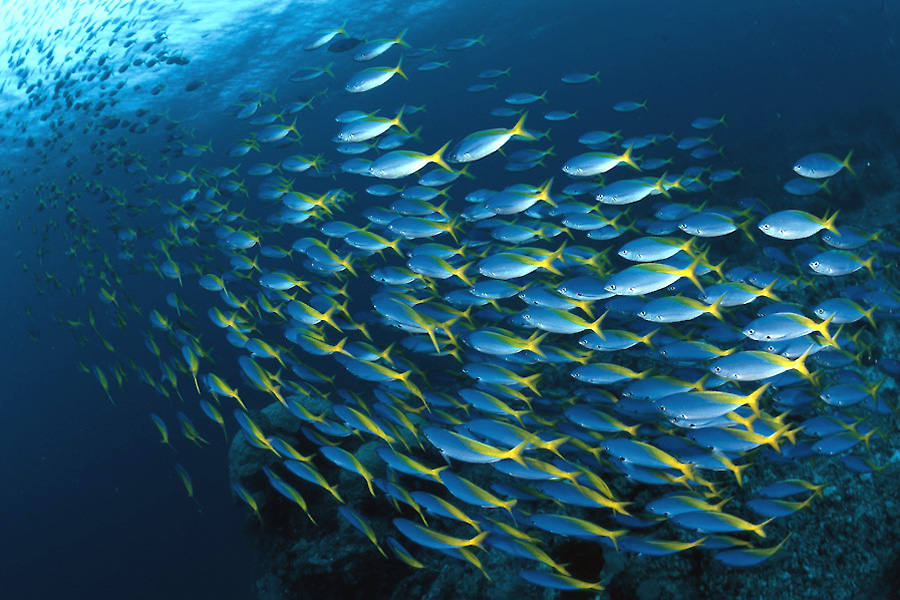
\includegraphics[width=0.4\textwidth]{images/technische_grundlagen/fischschwarm.jpg}
	\end{center}
	\caption{Fischschwarm}
	\label{fig:fischschwarm}
\end{wrapfigure}

\noindent
\paragraph{Ein Fischschwarm}
ist hierfür eines der bekanntesten Beispiele, indem die einzelnen Individuen des Schwarmes sich so verhalten, als würden sie wie ein einzelnes Tier agieren. Dabei setzt jeder Fisch feste Regeln um, die zur Umsetzung eines Schwarmverhaltens führen.%\footnote{\citep[vgl.][Schwarmverhalten]{Spektrum.SchwarmverhaltenKompaktlexikon}
\begin{enumerate}
	\item Folge deinem Vordermann
	\item Behalte die Geschwindigkeit deines Nachbarn bei
\end{enumerate}
\noindent
Die wichtigste Rolle spielt hierbei der Schwellenwert zur Steuerung des Schwarms durch einzelne Teilnehmer. Da jedes Individuum den Schwarm durch seine Bewegung beeinflusst, existiert ein Schwellenwert, der sich einer Mindestanzahl von etwa fünf Prozent richtet, durch die der Schwarm gesteuert werden kann. Somit reagieren die Fische ausschließlich auf die Mehrheit und der Schwarm lässt sich nicht durch eine Minderheit Fehlsteuern. Dieses Szenario lässt im Sinne von Veranstaltungen auf Menschen übertragen, um zu festzustellen an welchen Positionen Sicherheitspersonal positioniert werden muss, um einen geregelten Ablauf zu gewährleisten.%\footnote{\citep[vgl.][Schwarmverhalten]{Spektrum.SchwarmverhaltenKompaktlexikon}
\begin{wrapfigure}{r}{0.45\textwidth}
	\begin{center}
		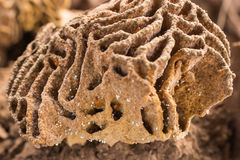
\includegraphics[width=0.4\textwidth]{images/technische_grundlagen/termitenschwarm.jpg}
	\end{center}
	\caption{Termitenschwarm}
	\label{fig:termitenschwarm}
\end{wrapfigure}

\noindent
\paragraph{Ein Termitenschwarm} geht nach dem Prinzip der Stigmergie vor, wie andere Insekten, die vorwiegend in einem Staat leben. Dabei kommunizieren die einzelnen Individuen indirekt über die Beeinflussung ihrer direkten Umgebung, wie dem Hinterlassen von Spuren als Merkmale. Dieses Prinzip ermöglicht auch den kleinsten und primitivsten Organismen einen evolutionären Vorteil zu erlagen, indem sie sich nicht allein den Gefahren stellen, sondern in einer großen Masse zusammenarbeiten.\\
Dies ermöglicht das Bauen riesiger Nester, indem die Insekten ihren inneren Plan, mit ihrer aktuellen Umgebung vergleichen und dadurch intuitiv erkennen, welche Arbeit sie zu erledigen haben.%\footnote{\citep[vgl.][Schwarmverhalten]{Spektrum.SchwarmverhaltenKompaktlexikon} 
	Der Ablauf ist dabei folgender:
\begin{enumerate}
	\item Erkennen
	\item Analysieren
	\item Reagieren
\end{enumerate}
Dieses Prinzip lässt sich durch festlegen von Regeln auf Roboterschwärme abbilden, um wie Insekten vollkommen autonom Gebäude und andere Objekte zu errichten. Zudem lässt sich dadurch eine indirekte Kommunikation und Zusammenarbeit zwischen Verschiedenartigen Robotern realisieren.%\footnote{\citep[vgl.][Schwarmverhalten]{Spektrum.SchwarmverhaltenKompaktlexikon}

\subsubsection{Szenarien}

Zur Umsetzung verschiedener Schwarmverhalten lassen sich nützliche Teile der Tierwelt auf Roboter abstrahieren, um eine Zusammenarbeit der einzelnen Individuen effizienter zu gestalten. Hierbei werden meist mehrere Basisszenarien eingesetzt, die einerseits die Kommunikation, oder Abläufe verbessern.\\
Für die Umsetzung der Kommunikation der einzelnen Teilnehmer existieren zwei verschiedene Möglichkeiten, einerseits eine direkt, oder indirekte Kommunikation. Dabei kann bei einer direkten Kommunikation auf die bekannten Kommunikationsmittel zurückgegriffen werden und über ein existierendes Netzwerk kommuniziert werden. Bei einer indirekte Kommunikation analysiert der Roboter dagegen seine direkte Umgebung, um daraus Veränderungen zu registrieren und entsprechend darauf zu reagieren. Dabei wird bei einer Umsetzung zur Implementierung folgend vorgegangen:
\begin{enumerate}
	\item Datenerfassung durch Sensorik
	\item Datenauswertung
	\item Vergleich der Datensätze
	\item Reaktion und Ausführung
\end{enumerate}



1. Separation

2. Aligment

3. Cohesion

4. Ausseneinflüsse
